% !TeX root = ../analisi_2.tex

\section{Funzioni implicite ed estremi vincolati}

\subsection{Teorema del Dini (o delle funzioni implicite)}

\begin{example}[ES 1]
Considero $F(x, y) = 0$, ovvero $x^2 + y^2 = 0$.

\begin{center}
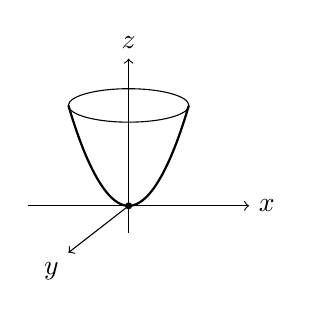
\begin{tikzpicture}[scale=0.85]
    \draw[->] (-1.5,0) -- (1.8,0) node[right] {$x$};
    \draw[->] (0,-0.4) -- (0,2.2) node[above] {$z$};
    \draw[->] (0,0) -- (-0.9,-0.7) node[below left] {$y$};
    \draw[thick] (-0.9,1.5) parabola bend (0,0) (0.9,1.5);
    \draw (0,1.5) ellipse (0.9 and 0.25);
    \fill (0,0) circle (1.5pt);
\end{tikzpicture}
\end{center}

\[
Z = \{ (x, y) \in \mathbb{R}^2 : F(x, y) = 0 \} = \{ (0, 0) \}
\]
Il problema è: $\exists g(x) : Z = \gamma(x) = (x, g(x))$? \pencilnote{($Z$ è il sostegno di una curva cartesiana?)}

In questo caso, non ha senso porsi questa domanda \pencilnote{(perché ho un solo punto)}.
\end{example}

\begin{example}[ES 2]
$F(x, y) = x^2 - y^2$, \qquad $F(x, y) = 0$.

\begin{center}
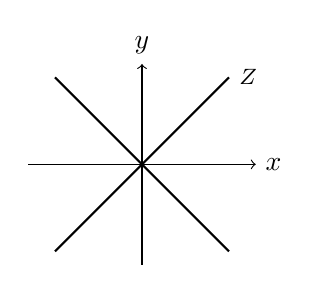
\begin{tikzpicture}[scale=0.85]
    \draw[->] (-1.7,0) -- (1.7,0) node[right] {$x$};
    \draw[->] (0,-1.5) -- (0,1.5) node[above] {$y$};
    \draw[thick] (-1.3,-1.3) -- (1.3,1.3) node[right] {\footnotesize $Z$};
    \draw[thick] (-1.3,1.3) -- (1.3,-1.3);
\end{tikzpicture}
\end{center}

$Z$ non è un grafico, ma se considero punto per punto (in un intorno) ho un grafico, ma nell'origine no!

Cosa li distingue?
\end{example}

\begin{example}[ESE 3]
$F(x, y) = x^2 + y^2 - 1$, \qquad $F(x, y) = 0$.

\begin{center}
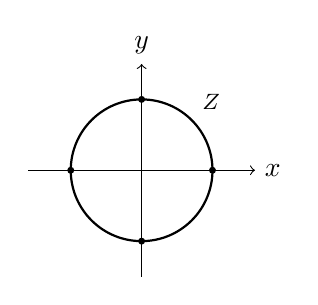
\begin{tikzpicture}[scale=0.9]
    \draw[->] (-1.6,0) -- (1.6,0) node[right] {$x$};
    \draw[->] (0,-1.5) -- (0,1.5) node[above] {$y$};
    \draw[thick] (0,0) circle (1.0);
    \node[above right] at (0.72,0.72) {\footnotesize $Z$};
    \fill (1,0) circle (1.4pt);
    \fill (-1,0) circle (1.4pt);
    \fill (0,1) circle (1.4pt);
    \fill (0,-1) circle (1.4pt);
\end{tikzpicture}
\end{center}

Anche qui $Z$ non è un grafico, ma localmente posso. Ad esempio in $P$ (nel 1° quadrante) potevo vedere il grafico (locale) sia come $g(x)$ che come $g(y)$; qui posso tranne nelle intersezioni con gli assi poiché ``fissata'' una variabile ottengo $2$ valori dell'altra.
\end{example}

\begin{theorem}[Teorema del Dini (o delle funzioni implicite)]
Sia $F : A \subseteq \mathbb{R}^2 \to \mathbb{R}$, $A \neq \emptyset$, aperto.

Sia $F \in C^1(A)$, sia $(x_0, y_0) \in A$ e t.c.:
\[
\begin{cases}
F(x_0, y_0) = 0 & \text{(ovvia)} \\
\nabla F(x_0, y_0) \neq (0, 0)
\end{cases}
\]
\pencilnote{(postilla: questo mi assicura ad esempio che in $Q$ si forma una curva)}

Allora $\exists I_\delta(x_0), I_\sigma(y_0)$ t.c. l'insieme
\[
Z = \underbrace{\{ (x, y) \in I_\delta(x_0) \times I_\sigma(y_0) : F(x, y) = 0 \}}_{Q}
\]
coincide con il grafico di una funzione:

\begin{center}
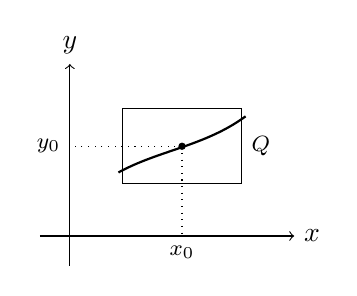
\begin{tikzpicture}[scale=0.95]
    \draw[->] (-0.4,0) -- (3.0,0) node[right] {$x$};
    \draw[->] (0,-0.4) -- (0,2.3) node[above] {$y$};
    \draw (0.7,0.7) rectangle (2.3,1.7);
    \node[right] at (2.3,1.2) {\footnotesize $Q$};
    \draw[thick] (0.65,0.85) .. controls (1.2,1.15) and (1.8,1.2) .. (2.35,1.6);
    \fill (1.5,1.2) circle (1.4pt);
    \draw[dotted] (1.5,1.2) -- (1.5,0) node[below] {\footnotesize $x_0$};
    \draw[dotted] (1.5,1.2) -- (0,1.2) node[left] {\footnotesize $y_0$};
\end{tikzpicture}
\end{center}

\begin{enumerate}
    \item Se $F_x(x_0, y_0) \neq 0$ allora $\exists! x = h(y)$ t.c. $F(h(y), y) = 0$ $\forall y \in I_\sigma(y_0) \implies Z$ è il grafico di $h$ nell'intorno.
    \item Se $F_y(x_0, y_0) \neq 0$ allora $\exists! y = g(x)$ t.c. $F(x, g(x)) = 0$ $\forall x \in I_\delta(x_0) \implies Z$ è il grafico di $g$ nell'intorno.
\end{enumerate}
\pencilnote{(Es. $F = ax + by + c$, $\nabla F = (a, b)$, se $b = F_y = 0 \implies$ non posso scrivere $y = g(x) = mx + q$. Ogni cosa sai già ma adesso è chiaro.)}

$h$ e $g$ si dicono definite ``implicitamente'' da $F(x, y) = 0$ al punto $(x_0, y_0)$, e si dicono \underline{funzioni implicite}.

Inoltre $h, g \in C^1$ e risulta:
\[
h'(y) = -\frac{F_y(h(y), y)}{F_x(h(y), y)}, \qquad g'(x) = -\frac{F_x(x, g(x))}{F_y(x, g(x))}
\]
\end{theorem}

\begin{proof}
Ovviamente $h(y_0) = x_0$, $g(x_0) = y_0$.

Dimostriamo la (2) \pencilnote{(la (1) è analoga)}.

Hp: $\begin{cases} F(x_0, y_0) = 0 \\ F_y(x_0, y_0) \neq 0 \end{cases} \implies$ (devo dim.) $\exists I_\delta(x_0), I_\sigma(y_0) : \exists! g(x), \ g : I_\delta(x_0) \to I_\sigma(y_0) \mid F(x, g(x)) = 0$.

Più precisamente, si dimostra che:
\begin{enumerate}
    \item $\exists g(x) : I_\delta(x_0) \to I_\sigma(y_0)$
    \item $g(x_0) = y_0$
    \item $g \in C^1$, \qquad $g'(x) = -\dfrac{F_x(x, g(x))}{F_y(x, g(x))}$
\end{enumerate}

%--------------------------------------------------------------
\medskip
\noindent\textbf{Passo 1: esistenza e unicità di $g$ (punti (1) e (2)).}

\begin{center}
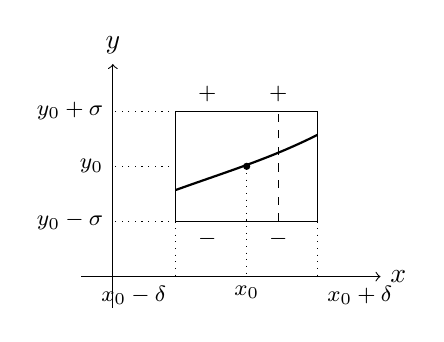
\begin{tikzpicture}[scale=1.0]
    \draw[->] (-0.4,0) -- (3.4,0) node[right] {$x$};
    \draw[->] (0,-0.4) -- (0,2.7) node[above] {$y$};
    \draw (0.8,0.7) rectangle (2.6,2.1);
    \draw[thick] (0.8,1.1) .. controls (1.5,1.35) and (2.0,1.5) .. (2.6,1.8);
    \draw[dashed] (2.1,0.7) -- (2.1,2.1);
    \fill (1.7,1.4) circle (1.3pt);
    \draw[dotted] (1.7,1.4) -- (1.7,0) node[below] {\footnotesize $x_0$};
    \draw[dotted] (0.8,0.7) -- (0.8,0) node[below left] {\footnotesize $x_0 - \delta$};
    \draw[dotted] (2.6,0.7) -- (2.6,0) node[below right] {\footnotesize $x_0 + \delta$};
    \draw[dotted] (0.8,1.4) -- (0,1.4) node[left] {\footnotesize $y_0$};
    \draw[dotted] (0.8,2.1) -- (0,2.1) node[left] {\footnotesize $y_0 + \sigma$};
    \draw[dotted] (0.8,0.7) -- (0,0.7) node[left] {\footnotesize $y_0 - \sigma$};
    \node[above] at (1.2,2.1) {\footnotesize $+$};
    \node[above] at (2.1,2.1) {\footnotesize $+$};
    \node[below] at (1.2,0.7) {\footnotesize $-$};
    \node[below] at (2.1,0.7) {\footnotesize $-$};
\end{tikzpicture}
\end{center}

\begin{itemize}
    \item Essendo $F_y(x_0, y_0) \neq 0 \implies$ ha un segno, supponiamo $F_y(x_0, y_0) > 0$.
    \item Per il T.P.S., $\exists$ un intorno del tipo $I_\sigma(x_0) \times I_\sigma(y_0) \subseteq A$ t.c. $F_y(x, y) > 0$ $\forall (x, y) \in I_\sigma(x_0) \times I_\sigma(y_0)$ \pencilnote{(creo il quadrato con $F_y > 0$)}.
    \item \pencilnote{(Costruisco i segni su un punto dei due lati)} Fissiamo $x_0$ e considero $F(x_0, y) = f(y)$ $\nearrow$ (st. crescente).
    \item Quindi essendo $f'(y) > 0 \implies F(x_0, y_0 - \sigma) < 0$ e $F(x_0, y_0 + \sigma) > 0$.
    \item Quindi per il TPS $\exists \delta \le \sigma$ t.c. $F(x, y_0 + \sigma) > 0$ in $I_\delta(x_0)$ e $F(x, y_0 - \sigma) < 0$ in $I_\delta(x_0)$ \pencilnote{(prolungo per tutti i lati)}.
    \item Sia $x \in I_\delta(x_0)$:
    \[
    F(x, y_0 - \sigma) \cdot F(x, y_0 + \sigma) < 0 \qquad \text{per costruzione.}
    \]
    Se riguardo $F(x, y)$ come sola funzione di $y$ nell'intervallo $[y_0 - \sigma, y_0 + \sigma]$, \pencilnote{(per il teorema degli zeri e la stretta monotonia)}:
    \[
    \exists! g(x) : f(g(x)) = 0 \implies \exists! g(x) : F(x, g(x)) = 0.
    \]
\end{itemize}

%--------------------------------------------------------------
\medskip
\noindent\textbf{Passo 2: $g \in C^1$ e formula della derivata (punto (3)).}

Per la derivata \pencilnote{(per averla devo avere $g \in C^1$)}:
\[
\langle \nabla F(x, g(x)), (1, g'(x)) \rangle = 0 \iff F_x(x, g(x)) + g'(x) F_y(x, g(x)) = 0
\]

La (3) si dim. calcolando il rapp. incr.:
\[
x, \bar{x} \in I_\delta(x_0) \to \frac{g(x) - g(\bar{x})}{x - \bar{x}} \qquad \text{\pencilnote{($\implies$ non conosco $g(x) \implies$ uso $F!$)}}
\]
$\implies F(x, g(x)) = F(\bar{x}, g(\bar{x})) = 0 \implies$ uso Lagrange:

\begin{center}
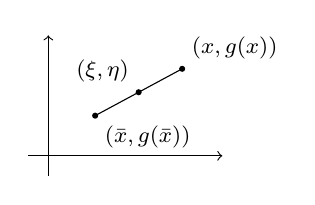
\begin{tikzpicture}[scale=0.85]
    \draw[->] (-0.3,0) -- (2.6,0);
    \draw[->] (0,-0.3) -- (0,1.8);
    \coordinate (Q) at (0.7,0.6);
    \coordinate (P) at (2.0,1.3);
    \coordinate (M) at (1.35,0.95);
    \draw (Q) -- (P);
    \fill (Q) circle (1.3pt) node[below right] {\footnotesize $(\bar{x}, g(\bar{x}))$};
    \fill (P) circle (1.3pt) node[above right] {\footnotesize $(x, g(x))$};
    \fill (M) circle (1.3pt) node[above left] {\footnotesize $(\xi, \eta)$};
\end{tikzpicture}
\end{center}

\begin{equation*}
F(x, g(x)) - F(\bar{x}, g(\bar{x})) = F_x(\xi, \eta)(x - \bar{x}) + F_y(\xi, \eta)(g(x) - g(\bar{x})) = 0 \tag{$*$}
\end{equation*}
$(\xi, \eta)$ si trova sul segmento di estremi $P(x, g(x))$, $Q = (\bar{x}, g(\bar{x}))$:
\[
\xi \in [x, \bar{x}], \quad \eta \in [g(x), g(\bar{x})] \qquad \xi \to \bar{x} \text{ se } x \to \bar{x}
\]
$\eta \to ?$ se $x \to \bar{x}$, ovvero $\boxed{g(x) \to g(\bar{x}) \text{ se } x \to \bar{x}}$? \pencilnote{($g$ è continua?)}

Uso $(*)$:
\[
g(x) - g(\bar{x}) = \frac{-F_x(\xi, \eta)(x - \bar{x})}{F_y(\xi, \eta)} \implies \text{passo ai moduli:}
\]
\[
|g(x) - g(\bar{x})| = \frac{|F_x(\xi, \eta)|}{|F_y(\xi, \eta)|} \underbrace{|x - \bar{x}|}_{\to 0}
\]
\pencilnote{$\dfrac{|F_x(\xi, \eta)|}{|F_y(\xi, \eta)|}$: la chiamo $f(x, y) \to$ non devo avere forma indeterminata; è continua (perché $F_y > 0$) in un compatto $\implies$ uso Weierstrass $\implies \exists \max_Q f(x, y) = M$.}

Dunque
\[
|g(x) - g(\bar{x})| = \left| \frac{F_x(\xi, \eta)}{F_y(\xi, \eta)} \right| |x - \bar{x}| \le M \underbrace{|x - \bar{x}|}_{\to 0} \implies g(x) \to g(\bar{x})
\]
Quindi $g$ è continua in $\bar{x} \implies$
\[
\frac{g(x) - g(\bar{x})}{x - \bar{x}} = -\frac{F_x(\xi, \eta)}{F_y(\xi, \eta)} \to -\frac{F_x(\bar{x}, g(\bar{x}))}{F_y(\bar{x}, g(\bar{x}))}
\]
\end{proof}

\begin{oss}
In $(x_0, y_0) \implies g'(x_0) = -\dfrac{F_x(x_0, y_0)}{F_y(x_0, y_0)}$.

\begin{center}
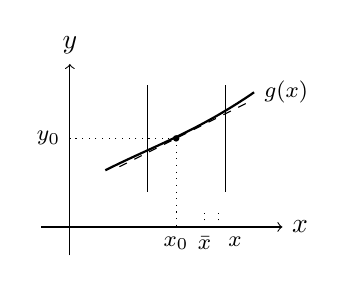
\begin{tikzpicture}[scale=0.9]
    \draw[->] (-0.4,0) -- (3.0,0) node[right] {$x$};
    \draw[->] (0,-0.4) -- (0,2.3) node[above] {$y$};
    \draw (1.1,0.5) -- (1.1,2.0);
    \draw (2.2,0.5) -- (2.2,2.0);
    \draw[thick] (0.5,0.8) .. controls (1.2,1.15) and (1.8,1.35) .. (2.6,1.9) node[right] {\footnotesize $g(x)$};
    \draw[dashed] (0.7,0.85) -- (2.5,1.75);
    \fill (1.5,1.25) circle (1.3pt);
    \draw[dotted] (1.5,1.25) -- (1.5,0) node[below] {\footnotesize $x_0$};
    \draw[dotted] (1.5,1.25) -- (0,1.25) node[left] {\footnotesize $y_0$};
    \draw[dotted] (1.9,0) node[below] {\footnotesize $\bar{x}$} -- (1.9,0.2);
    \draw[dotted] (2.1,0) node[below right] {\footnotesize $x$} -- (2.1,0.2);
\end{tikzpicture}
\end{center}
\pencilnote{Retta tang. (Dini): $y = g(x_0) + g'(x_0)(x - x_0)$.}
\end{oss}

\begin{esercizio}[ESE 1]
$F(x, y) = x^2 + y^2$. In $(0, 0)$ si applica Dini?
\[
\nabla F(x, y) = (2x, 2y)\big|_{(0, 0)} = (0, 0) \implies \text{Dini non si applica.}
\]
\end{esercizio}

\begin{esercizio}[ESE 2]
$F(x, y) = x^2 - y^2$
\[
\begin{cases}
F_x = 2x = 0 \\
F_y = -2y = 0
\end{cases}
\iff (0, 0) \implies \text{in questo punto non si applica Dini (negli altri sì).}
\]
\begin{center}
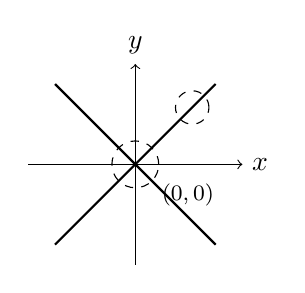
\begin{tikzpicture}[scale=0.85]
    \draw[->] (-1.6,0) -- (1.6,0) node[right] {$x$};
    \draw[->] (0,-1.5) -- (0,1.5) node[above] {$y$};
    \draw[thick] (-1.2,-1.2) -- (1.2,1.2);
    \draw[thick] (-1.2,1.2) -- (1.2,-1.2);
    \draw[dashed] (0,0) circle (0.35);
    \node[below right] at (0.25,-0.15) {\footnotesize $(0, 0)$};
    \draw[dashed] (0.85,0.85) circle (0.25);
\end{tikzpicture}
\end{center}
In $(0, 0)$ non ho un grafico, negli altri punti ho la ``doppia scelta''.
\end{esercizio}

\begin{esercizio}[ESE 3]
$F(x, y) = x^2 + y^2 - 1$
\[
\begin{cases}
F_x = 2x = 0 \\
F_y = 2y = 0
\end{cases}
\iff (0, 0) \to \text{punto che non è uno zero} \implies \text{Dini vale in tutti gli zeri.}
\]
\begin{center}
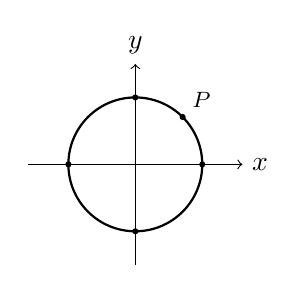
\begin{tikzpicture}[scale=0.85]
    \draw[->] (-1.6,0) -- (1.6,0) node[right] {$x$};
    \draw[->] (0,-1.5) -- (0,1.5) node[above] {$y$};
    \draw[thick] (0,0) circle (1.0);
    \fill (1,0) circle (1.3pt);
    \fill (-1,0) circle (1.3pt);
    \fill (0,1) circle (1.3pt);
    \fill (0,-1) circle (1.3pt);
    \fill (0.707,0.707) circle (1.3pt) node[above right] {\footnotesize $P$};
\end{tikzpicture}
\end{center}
Noto che nelle intersezioni con gli assi (ad esempio $(1, 0)$) ho una delle due comp. di $\nabla F$ nulla (nel punto $(1, 0)$: $F_y(1, 0) = 0$). Nonostante ciò se considero $F(x, 0) = 0$ ottengo $F(x, 0) = x^2 - 1 = 0 \implies$ sono gli $x = \pm 1$, cioè $(1, 0)$ e $(-1, 0)$ ($+$ discorso analogo su $y$).
\end{esercizio}

\begin{oss}
\begin{enumerate}
    \item $y = g(x_0) + g'(x_0)(x - x_0) \implies y = y_0 - \dfrac{F_x(x_0, y_0)}{F_y(x_0, y_0)}(x - x_0)$ \quad \pencilnote{(retta tang. in un punto)}
    \[
    \implies \boxed{F_x(x_0, y_0)(x - x_0) + F_y(x_0, y_0)(y - y_0) = 0} \qquad \text{\pencilnote{retta tang. a $g$ nel punto $(x_0, y_0)$}}
    \]
    \item $f(x, y) = c \implies f(x, y) - c = 0 \implies F(x, y) = 0$, $f \in C^1$, con $F(x_0, y_0) = 0$ e $\nabla f(x_0, y_0) \neq (0, 0)$.

    Vale Dini: $\exists g(x) : F(x, g(x)) = 0$ oppure $\exists h(y) : F(h(y), y) = 0$.
\end{enumerate}
\pencilnote{($P(x) = F(x, g(x)) = 0 \implies P'(x) = \langle \nabla F(x, g(x)), (1, g') \rangle = 0$: lo capisco calcolando $g'$).}
\end{oss}

\subsection{Punti singolari e regolari}

\begin{definition}[Punti singolari e regolari]
Sia
\[
C = \{ \text{punti critici} \} = \{ (x, y) : \nabla F(x, y) = (0, 0) \}
\]
\[
Z = \{ \text{zeri} \} = \{ (x, y) : F(x, y) = 0 \}
\]
Definiamo:
\[
Z \cap C = \{ \text{\underline{punti singolari}} \}, \qquad Z \setminus C = \{ \text{\underline{punti regolari}} \}
\]
\end{definition}

\begin{esercizio}[EXE]
$F(x, y) = x^2(1 + 4x) - y^2$ \pencilnote{$(= x^2 + 4x^3 - y^2)$}. Studiare i punti singolari e regolari.

$\nabla F = (F_x, F_y)$:
\[
\begin{cases}
F_x = 2x + 12x^2 = 0 \iff x = 0 \ \lor \ x = -\dfrac{1}{6} \\
F_y = -2y = 0 \iff y = 0
\end{cases}
\to (0, 0), \ \left(-\frac{1}{6}, 0\right) \implies \text{sono zeri?}
\]
\begin{itemize}
    \item $(0, 0) \in Z$
    \item $F\left(-\dfrac{1}{6}, 0\right) = \dfrac{1}{36}\left(1 - \dfrac{2}{3}\right) \neq 0$
\end{itemize}
$\implies (0, 0) \in Z \cap C =$ singolare.

Inoltre $\left(-\dfrac{1}{4}, 0\right) \notin C$, $\left(-\dfrac{1}{4}, 0\right) \in Z \implies \left(-\dfrac{1}{4}, 0\right) \in Z \setminus C$ regolare.
\end{esercizio}

\subsection{Estremi vincolati e moltiplicatori di Lagrange}

\begin{definition}
Sia $(\bar{x}, \bar{y}) \in Z = \{ (x, y) \in A : F(x, y) = 0 \}$, dove $F : A \subseteq \mathbb{R}^2 \to \mathbb{R}$, $A \neq \emptyset$, aperto, $F \in C^1$.

$(\bar{x}, \bar{y})$ si dice \underline{estremo vincolato} per $f : A \to \mathbb{R}$, $f \in C^1(A)$ \pencilnote{(serve dopo)} se $\exists I_\delta(\bar{x}, \bar{y})$ t.c.:
\begin{itemize}
    \item $f(\bar{x}, \bar{y}) \le f(x, y) \quad \forall (x, y) \in I_\delta(\bar{x}, \bar{y}) \cap Z$ \quad (min vincolato)
    \item $f(\bar{x}, \bar{y}) \ge f(x, y) \quad \forall (x, y) \in I_\delta(\bar{x}, \bar{y}) \cap Z$ \quad (max vincolato)
\end{itemize}
\begin{center}
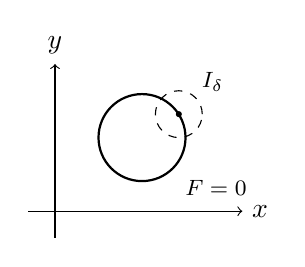
\begin{tikzpicture}[scale=0.85]
    \draw[->] (-0.4,0) -- (2.8,0) node[right] {$x$};
    \draw[->] (0,-0.4) -- (0,2.2) node[above] {$y$};
    \draw[thick] (1.3,1.1) circle (0.65);
    \node[below right] at (1.8,0.6) {\footnotesize $F = 0$};
    \draw[dashed] (1.85,1.45) circle (0.35);
    \fill (1.85,1.45) circle (1.3pt);
    \node[above right] at (2.05,1.65) {\footnotesize $I_\delta$};
\end{tikzpicture}
\end{center}
\pencilnote{OSS: può non essere estremo relativo.}
\end{definition}

\begin{oss}[Deduzione dei moltiplicatori di Lagrange]
Sia $f(x, y) : A \to \mathbb{R}$, $f \in C^1(A)$, $\{ F(x, y) = 0 \} = Z$.

Sia $(\bar{x}, \bar{y})$ un estremo vincolato \pencilnote{e che sia regolare} $\implies (\bar{x}, \bar{y}) \in Z$ e $f(x, y) - f(\bar{x}, \bar{y})$ ha segno in $I_\delta \cap Z$.

$\implies \text{Dini} \implies \exists y = g(x)$ funz. implicita t.c. $F(x, g(x)) = 0$ in $I_\delta(\bar{x})$ \pencilnote{($g(\bar{x}) = \bar{y}$)}.

$H(x) = f(x, g(x))$ ha in $\bar{x}$ un pto di estremo relativo $\implies H'(\bar{x}) = 0 \to$ Teo der. funz. comp. $\implies$
\[
H'(\bar{x}) = \langle \nabla f(\bar{x}, \bar{y}), (1, g'(\bar{x})) \rangle = 0, \qquad g'(\bar{x}) = -\frac{F_x(\bar{x}, \bar{y})}{F_y(\bar{x}, \bar{y})}
\]
\[
\implies \boxed{f_x(\bar{x}, \bar{y}) \cdot F_y(\bar{x}, \bar{y}) - f_y(\bar{x}, \bar{y}) F_x(\bar{x}, \bar{y}) = 0}
\]
Ovvero:
\[
\begin{vmatrix}
f_x(\bar{x}, \bar{y}) & f_y(\bar{x}, \bar{y}) \\
F_x(\bar{x}, \bar{y}) & F_y(\bar{x}, \bar{y})
\end{vmatrix} = 0 \iff \text{i due gradienti sono lin. dip.} \iff \exists \bar{\lambda} \text{ t.c. } \nabla f(\bar{x}, \bar{y}) = \bar{\lambda} \nabla F(\bar{x}, \bar{y})
\]
\[
\implies \begin{cases}
f_x(\bar{x}, \bar{y}) = \bar{\lambda} F_x(\bar{x}, \bar{y}) \\
f_y(\bar{x}, \bar{y}) = \bar{\lambda} F_y(\bar{x}, \bar{y}) \\
F(\bar{x}, \bar{y}) = 0
\end{cases}
\qquad \text{$\bar{\lambda}$ è detto \underline{moltiplicatore di Lagrange}.}
\]
Ponendo
\[
\mathcal{L}(x, y, \lambda) = f(x, y) - \lambda F(x, y)
\]
$\implies (\bar{x}, \bar{y}, \bar{\lambda})$ è punto critico di $\mathcal{L}(x, y, \lambda)$ \pencilnote{(le soluzioni del sistema sono i punti critici di $\mathcal{L}(x, y, \lambda)$)}.

$\mathcal{L}$ è detta \underline{Lagrangiana} \pencilnote{(il sistema è il gradiente di $\mathcal{L}$: $\nabla \mathcal{L}$)}.
\end{oss}

\begin{theorem}[Teorema dei moltiplicatori di Lagrange]
Sia $f \in C^1(A)$, $F \in C^1(A)$, $A \subseteq \mathbb{R}^2$, $A$ aperto.

Sia $(\bar{x}, \bar{y})$ un estremo vincolato per $f$ con vincolo $F(x, y) = 0$ e sia regolare.

Allora $\exists \bar{\lambda} \in \mathbb{R} : (\bar{x}, \bar{y}, \bar{\lambda})$ è un punto critico \pencilnote{(vero)} per la funzione $\mathcal{L}(x, y, \lambda)$ e $\lambda$ viene detto \underline{moltiplicatore di Lagrange}.
\end{theorem}

\begin{esercizio}[EXE]
$F(x, y) = x^2 - xy + y^2 - 1 = 0$, \qquad $f(x, y) = xy$.

Trovare gli estremi vincolati \pencilnote{(è chiuso e compatto, quindi su di esso esiste max e min per Weierstrass; è un'ellisse ruotata)}.

\[
\nabla F(x, y) = (0, 0) \iff \begin{cases} F_x = 0 \\ F_y = 0 \end{cases} \iff \begin{cases} 2x - y = 0 \\ -x + 2y = 0 \end{cases} \to (0, 0) \notin Z \implies \text{tutti gli zeri sono regolari.}
\]
\[
\mathcal{L}(x, y, \lambda) = f(x, y) - \lambda F(x, y) = xy - \lambda(x^2 - xy + y^2 - 1)
\]
\[
\begin{cases}
y - \lambda(2x - y) = 0 \\
x - \lambda(-x + 2y) = 0 \\
x^2 - xy + y^2 - 1 = 0
\end{cases}
\xrightarrow{\text{risolvo}}
\begin{aligned}
&(1, 1, 1) \\
&(-1, -1, 1) \\
&\left( \frac{1}{\sqrt{3}}, -\frac{1}{\sqrt{3}}, -\frac{1}{3} \right) \\
&\left( -\frac{1}{\sqrt{3}}, \frac{1}{\sqrt{3}}, -\frac{1}{3} \right)
\end{aligned}
\]
Trovo i valori valutando $f(1, 1)$, $f(-1, -1)$, $f\left(\frac{1}{\sqrt{3}}, -\frac{1}{\sqrt{3}}\right)$ e $f\left(-\frac{1}{\sqrt{3}}, \frac{1}{\sqrt{3}}\right)$.
\end{esercizio}
